\documentclass[journal, a4paper]{IEEEtran}

\usepackage[utf8x]{inputenc}
\usepackage[francais]{babel}

% some very useful LaTeX packages include:

%\usepackage{cite}      % Written by Donald Arseneau
                        % V1.6 and later of IEEEtran pre-defines the format
                        % of the cite.sty package \cite{} output to follow
                        % that of IEEE. Loading the cite package will
                        % result in citation numbers being automatically
                        % sorted and properly "ranged". i.e.,
                        % [1], [9], [2], [7], [5], [6]
                        % (without using cite.sty)
                        % will become:
                        % [1], [2], [5]--[7], [9] (using cite.sty)
                        % cite.sty's \cite will automatically add leading
                        % space, if needed. Use cite.sty's noadjust option
                        % (cite.sty V3.8 and later) if you want to turn this
                        % off. cite.sty is already installed on most LaTeX
                        % systems. The latest version can be obtained at:
                        % http://www.ctan.org/tex-archive/macros/latex/contrib/supported/cite/

\usepackage{graphicx}   % Written by David Carlisle and Sebastian Rahtz
                        % Required if you want graphics, photos, etc.
                        % graphicx.sty is already installed on most LaTeX
                        % systems. The latest version and documentation can
                        % be obtained at:
                        % http://www.ctan.org/tex-archive/macros/latex/required/graphics/
                        % Another good source of documentation is "Using
                        % Imported Graphics in LaTeX2e" by Keith Reckdahl
                        % which can be found as esplatex.ps and epslatex.pdf
                        % at: http://www.ctan.org/tex-archive/info/

%\usepackage{psfrag}    % Written by Craig Barratt, Michael C. Grant,
                        % and David Carlisle
                        % This package allows you to substitute LaTeX
                        % commands for text in imported EPS graphic files.
                        % In this way, LaTeX symbols can be placed into
                        % graphics that have been generated by other
                        % applications. You must use latex->dvips->ps2pdf
                        % workflow (not direct pdf output from pdflatex) if
                        % you wish to use this capability because it works
                        % via some PostScript tricks. Alternatively, the
                        % graphics could be processed as separate files via
                        % psfrag and dvips, then converted to PDF for
                        % inclusion in the main file which uses pdflatex.
                        % Docs are in "The PSfrag System" by Michael C. Grant
                        % and David Carlisle. There is also some information
                        % about using psfrag in "Using Imported Graphics in
                        % LaTeX2e" by Keith Reckdahl which documents the
                        % graphicx package (see above). The psfrag package
                        % and documentation can be obtained at:
                        % http://www.ctan.org/tex-archive/macros/latex/contrib/supported/psfrag/

%\usepackage{subfigure} % Written by Steven Douglas Cochran
                        % This package makes it easy to put subfigures
                        % in your figures. i.e., "figure 1a and 1b"
                        % Docs are in "Using Imported Graphics in LaTeX2e"
                        % by Keith Reckdahl which also documents the graphicx
                        % package (see above). subfigure.sty is already
                        % installed on most LaTeX systems. The latest version
                        % and documentation can be obtained at:
                        % http://www.ctan.org/tex-archive/macros/latex/contrib/supported/subfigure/

\usepackage{url}        % Written by Donald Arseneau
                        % Provides better support for handling and breaking
                        % URLs. url.sty is already installed on most LaTeX
                        % systems. The latest version can be obtained at:
                        % http://www.ctan.org/tex-archive/macros/latex/contrib/other/misc/
                        % Read the url.sty source comments for usage information.

%\usepackage{stfloats}  % Written by Sigitas Tolusis
                        % Gives LaTeX2e the ability to do double column
                        % floats at the bottom of the page as well as the top.
                        % (e.g., "\begin{figure*}[!b]" is not normally
                        % possible in LaTeX2e). This is an invasive package
                        % which rewrites many portions of the LaTeX2e output
                        % routines. It may not work with other packages that
                        % modify the LaTeX2e output routine and/or with other
                        % versions of LaTeX. The latest version and
                        % documentation can be obtained at:
                        % http://www.ctan.org/tex-archive/macros/latex/contrib/supported/sttools/
                        % Documentation is contained in the stfloats.sty
                        % comments as well as in the presfull.pdf file.
                        % Do not use the stfloats baselinefloat ability as
                        % IEEE does not allow \baselineskip to stretch.
                        % Authors submitting work to the IEEE should note
                        % that IEEE rarely uses double column equations and
                        % that authors should try to avoid such use.
                        % Do not be tempted to use the cuted.sty or
                        % midfloat.sty package (by the same author) as IEEE
                        % does not format its papers in such ways.

\usepackage{amsmath}    % From the American Mathematical Society
                        % A popular package that provides many helpful commands
                        % for dealing with mathematics. Note that the AMSmath
                        % package sets \interdisplaylinepenalty to 10000 thus
                        % preventing page breaks from occurring within multiline
                        % equations. Use:
%\interdisplaylinepenalty=2500
                        % after loading amsmath to restore such page breaks
                        % as IEEEtran.cls normally does. amsmath.sty is already
                        % installed on most LaTeX systems. The latest version
                        % and documentation can be obtained at:
                        % http://www.ctan.org/tex-archive/macros/latex/required/amslatex/math/



% Other popular packages for formatting tables and equations include:

%\usepackage{array}
% Frank Mittelbach's and David Carlisle's array.sty which improves the
% LaTeX2e array and tabular environments to provide better appearances and
% additional user controls. array.sty is already installed on most systems.
% The latest version and documentation can be obtained at:
% http://www.ctan.org/tex-archive/macros/latex/required/tools/

% V1.6 of IEEEtran contains the IEEEeqnarray family of commands that can
% be used to generate multiline equations as well as matrices, tables, etc.

% Also of notable interest:
% Scott Pakin's eqparbox package for creating (automatically sized) equal
% width boxes. Available:
% http://www.ctan.org/tex-archive/macros/latex/contrib/supported/eqparbox/

% *** Do not adjust lengths that control margins, column widths, etc. ***
% *** Do not use packages that alter fonts (such as pslatex).         ***
% There should be no need to do such things with IEEEtran.cls V1.6 and later.


% Your document starts here!
\begin{document}

% Define document title and author
	\title{Administration des réseaux}
	\author{Alexandre Kervadec
	\thanks{Professeur : A.Guermouche}}
	\markboth{Université de Bordeaux - Master 1 Informatique}{}
	\maketitle

% Write abstract here
\begin{abstract}
	Notes du cours d'administration des réseaux de A.Guermouche
\end{abstract}

% Each section begins with a \section{title} command
\section{Modèle TCP/IP}
	% \PARstart{}{} creates a tall first letter for this first paragraph
	\subsection{Le visage d'internet}
	\begin{itemize}
		\item Une construction à partir du "bas"
		\begin{itemize}
			\item réseau local (laboratoire, département)
			\item réseau local (campus, entreprise)
			\item réseau régional
			\item réseau national
			\item réseau mondial
		\end{itemize}
		\item 3 niveaux d'interconnexion
		\begin{itemize}
			\item postes de travail (ordinateur, terminal, ...)
			\item liaisons physiques (câble, fibre, RTC, ...)
			\item routeurs (équipement spécialisé, ordinateur, ...)
		\end{itemize}
	\end{itemize}
	C'est un ensemble de sous-réseaux indépendants (Autonomous System) et hétérogènes qui sont inter-connectés (organisation hiérarchique)
	
	\begin{figure}[!hbt]
		\begin{center}
		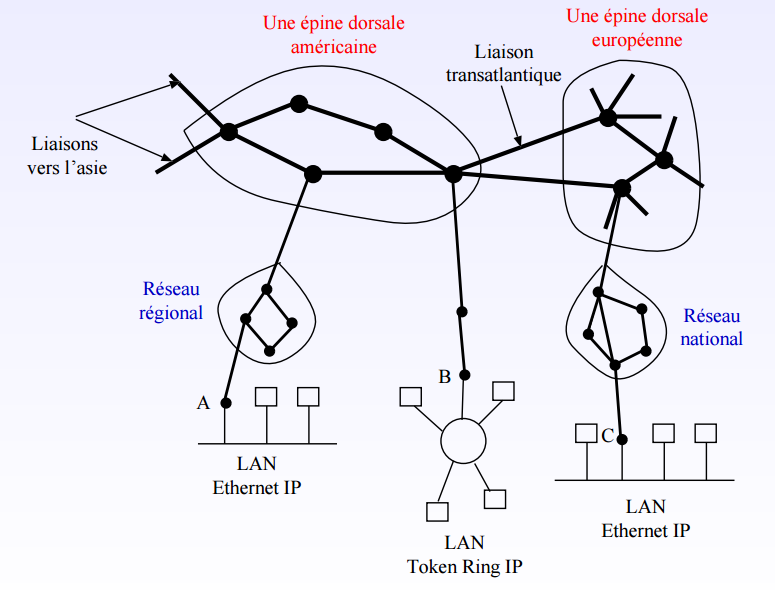
\includegraphics[width=\columnwidth]{orga_hier.png}
		\label{fig:orga_hier}
		\end{center}
	\end{figure}
	
	\subsection{Architecture TCP/IP}
	L'architecture TCP/IP est une version simplifiée du modèle OSI.
	\begin{itemize}
		\item \textbf{Application} : FTP, WWW, Telnet, SMTP, ...
		\item \textbf{Transport} : TCP, UDP (entre 2 processus aux extrémités)
		\begin{itemize}
			\item TCP : transfert fiable de données en mode connecté
			\item UDP : transfert non garanti de données en mode non-connecté
		\end{itemize}
		\item \textbf{Réseau} : IP (routage)
		\item \textbf{Physique} : transmission entre 2 sites
		\begin{itemize}
			\item TCP : Transport Control Protocol
			\item UDP : User Datagram Protocol
			\item IP : Internet Protocol
		\end{itemize}
 	\end{itemize}
	
	\begin{figure}[!hbt]
		\begin{center}
		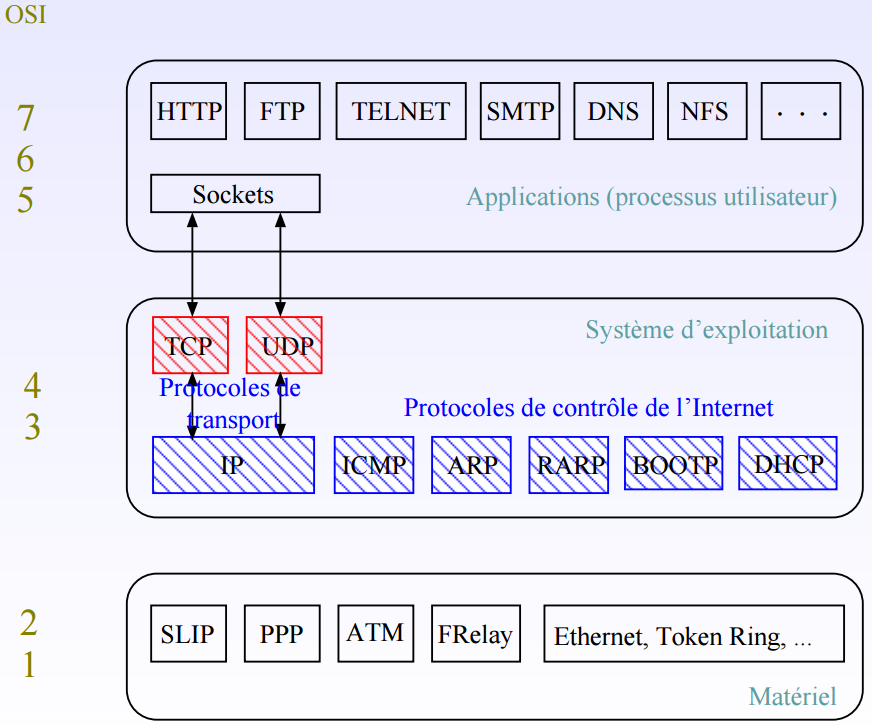
\includegraphics[width=\columnwidth]{archi_tcp_ip.png}
		\caption{Architecture TCP/IP}
		\label{fig:archi_tcp_ip}
		\end{center}
	\end{figure}
	
	\begin{figure}[!hbt]
		\begin{center}
		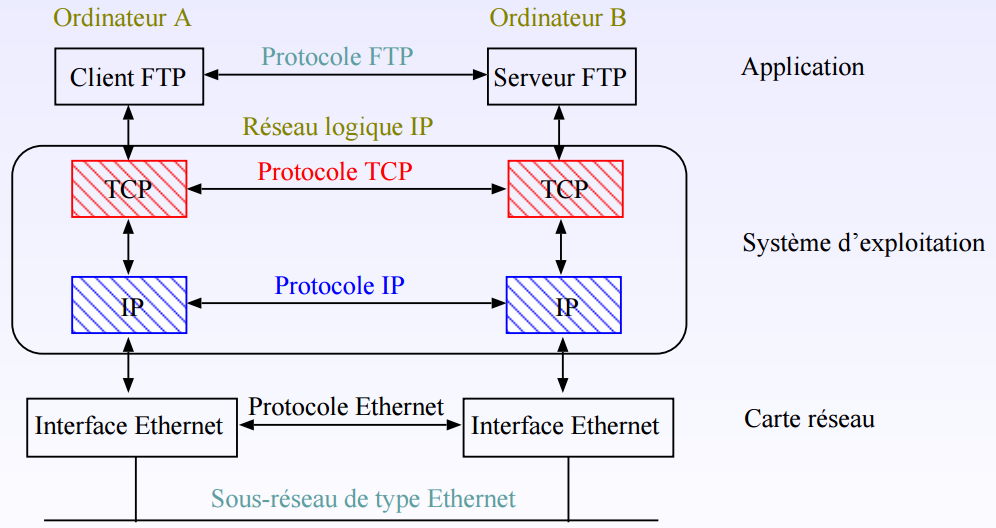
\includegraphics[width=\columnwidth]{sous_res_ip.png}
		\caption{Sous-réseau IP}
		\label{fig:sous_res_ip}
		\end{center}
	\end{figure}
	
	\newpage
	
	\begin{figure}[!hbt]
		\begin{center}
		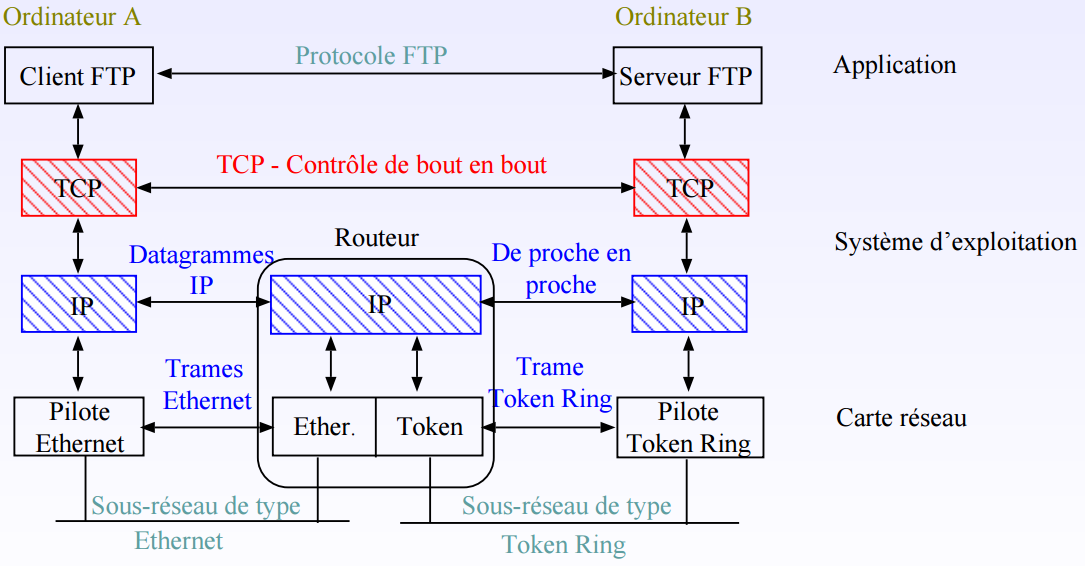
\includegraphics[width=\columnwidth]{hetero.png}
		\caption{Prise en compte de l'hétérogénéité}
		\label{fig:hetero}
		\end{center}
	\end{figure}
	
	\begin{figure}[!hbt]
		\begin{center}
		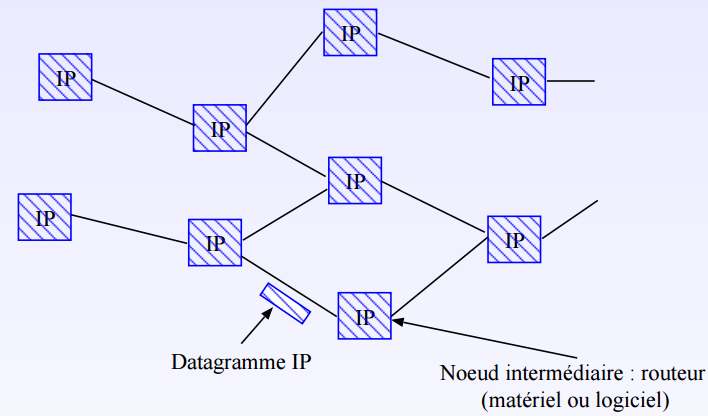
\includegraphics[width=\columnwidth]{comm.png}
		\caption{Couche réseau : communication entre machines}
		\label{fig:comm}
		\end{center}
	\end{figure}
	
	\subsection{Protocole IP}
	IP - Protocole d'interconnexion, best-effort
	\begin{itemize}
		\item acheminement de \textit{datagrammes} (mode \textit{non-connecté}
		\item peu de fonctionnalités
		\item pas de garanties, simple mais robuste (défaillance d’un noeud
intermédiaire)
	\end{itemize}
	
	\begin{figure}[!hbt]
		\begin{center}
		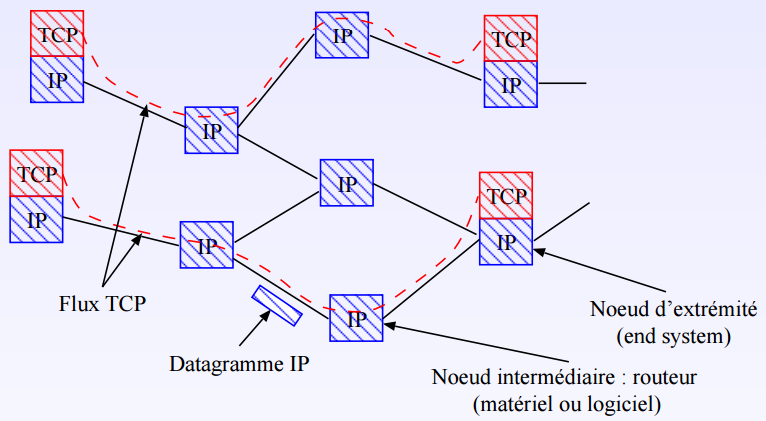
\includegraphics[width=\columnwidth]{comm2.png}
		\caption{Couche réseau : communication entre applications}
		\label{fig:comm2}
		\end{center}
	\end{figure}
	
	\subsection{Protocole TCP}
	TCP - Protocole de transport \textit{de bout en bout}
	\begin{itemize}
		\item uniquement présent aux \textit{extrémités}
		\item transport \textit{fiable} de \textit{segments} (mode \textit{connecté})
		\item protocole complexe (retransmission, gestion des erreurs, séquencement, ...)
	\end{itemize}
	
	\begin{figure}[!hbt]
		\begin{center}
		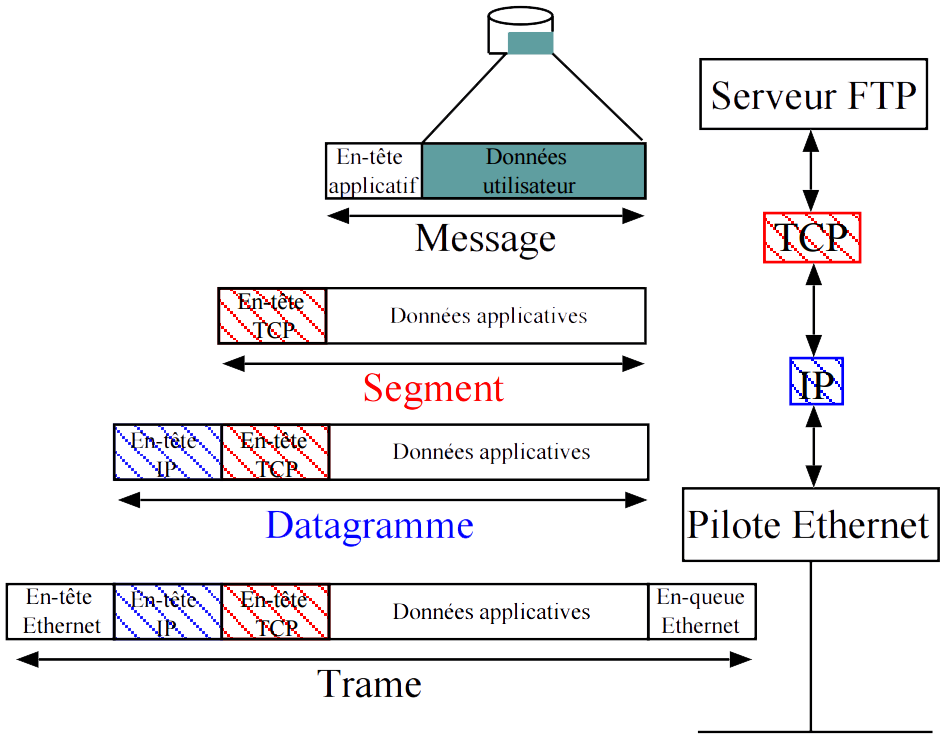
\includegraphics[width=\columnwidth]{archi_trame.png}
		\caption{Couche réseau : communication entre applications}
		\label{fig:archi_trame}
		\end{center}
	\end{figure}
	
	\begin{figure}[!hbt]
		\begin{center}
		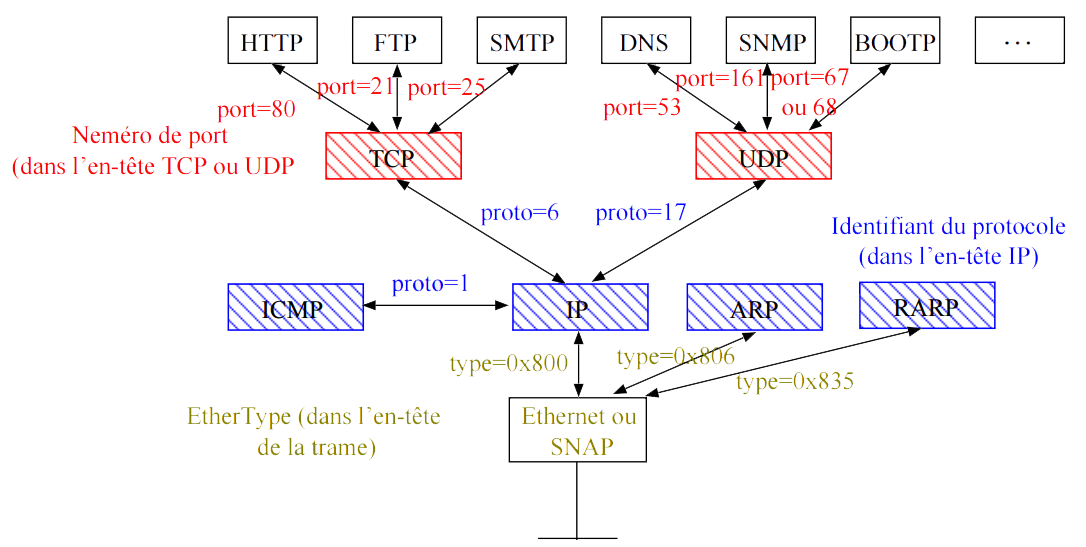
\includegraphics[width=\columnwidth]{id_proto.png}
		\caption{Identification des protocoles}
		\label{fig:id_proto}
		\end{center}
	\end{figure}
	
	\subsection{Identification des protocoles}
	
	\begin{itemize}
		\item Une adresse de transport = une adresse IP + un numéro de
port (16 bits) → adresse de socket
		\item Une connexion s’établit entre une socket source et une socket
destinataire → une connexion = un quintuplé (proto, src, port
src, dest, port dest)
		\item Deux connexions peuvent aboutir à la même socket
		\item Les ports permettent un multiplexage ou démultiplexage de
connexions au niveau transport
		\item Les ports inférieurs à 1024 sont appelés \textit{ports réservés}
	\end{itemize}
	
	\subsection{Protocole UDP}
	UDP (RFC 768) - User Datagram Protocol :
	
	\begin{itemize}
		\item protocole de transport le plus simple
		\item service de type best-effort (comme IP)
		\begin{itemize}
			\item les segments UDP peuvent être perdus
			\item les segments UDP peuvent arriver dans le désordre
		\end{itemize}
		\item  mode non connecté : chaque segment UDP est traité
indépendamment des autres
	\end{itemize}
	
	Pourquoi un service non fiable sans connexion ?
	
	\begin{itemize}
		\item simple donc rapide (pas de délai de connexion, pas d’état
entre émetteur/récepteur)
		\item petit en-tête donc économie de bande passante
		\item sans contrôle de congestion donc UDP peut émettre aussi
rapidement qu’il le souhaite
	\end{itemize}
	
	Les utilisations de l'UDP :
	
	\begin{itemize}
		\item Performance sans garantie de délivrance
		\item Souvent utilisé pour les applications multimédias
		\begin{itemize}
			\item tolérantes aux pertes
			\item sensibles au débit
		\end{itemize}
		\item Autres utilisations d’UDP
		\begin{itemize}
			\item applications qui envoient peu de données et qui ne nécessitent
pas un service fiable
			\item exemples : DNS, SNMP, BOOTP/DHCP
		\end{itemize}
		\item Transfert fiable sur UDP
		\begin{itemize}
			\item ajouter des mécanismes de compensation de pertes (reprise
sur erreur) au niveau applicatif
			\item mécanismes adaptés à l’application
		\end{itemize}
	\end{itemize}
	
	
	\subsection{Protocole TCP}
	Transport Control Protocol (RFC 793, 1122, 1323, 2018, 2581)
	Transport fiable en mode connecté :
	\begin{itemize}
		\item point à point, bidirectionnel : entre deux adresses de transport
(@IP src, port src) → (@IP dest, port dest)
		\item transporte un flot d’octets (ou flux)
		\begin{itemize}
			\item l’application lit/écrit des octets dans un tampon
		\end{itemize}
		\item assure la délivrance des données en séquence
		\item contrôle la validité des données reçues
		\item organise les reprises sur erreur ou sur temporisation
		\item réalise le contrôle de flux et le contrôle de congestion (à l’aide
d’une fenêtre d’émission)
	\end{itemize}
	
	\subsection{Exemples de protocole applicatif}
	\begin{itemize}
		\item HTTTP - HyperText Transport Protocol
		\begin{itemize}
			\item protocole du web
			\item échange de requête/réponse entre un client et u
serveur web
		\end{itemize}
		\item FTP - File Tranfer Protocol
		\begin{itemize}
			\item protocole de manipulation de fichiers distants
			\item tranfert, suppression, création, ...
		\end{itemize}
		\item TELNET - TELetypewriter Network Protocol
		\begin{itemize}
			\item système de terminal virtuel
			\item permet l'ouverture d'une session distante
		\end{itemize}
		\item DNS - Domain Name System
		\begin{itemize}
			\item assure la correspondance entre un nom
symbolique et une adresse Internet (adresse IP)
			\item bases de données réparties sur le globe
		\end{itemize}
	\end{itemize}
	
	\newpage



% Now we need a bibliography:
\begin{thebibliography}{5}

	%Each item starts with a \bibitem{reference} command and the details thereafter.
	\bibitem{HOP96} % Transaction paper
	J.~Hagenauer, E.~Offer, and L.~Papke. Iterative decoding of binary block
	and convolutional codes. {\em IEEE Trans. Inform. Theory},
	vol.~42, no.~2, pp.~429–-445, Mar. 1996.

	\bibitem{MJH06} % Conference paper
	T.~Mayer, H.~Jenkac, and J.~Hagenauer. Turbo base-station cooperation for intercell interference cancellation. {\em IEEE Int. Conf. Commun. (ICC)}, Istanbul, Turkey, pp.~356--361, June 2006.

	\bibitem{Proakis} % Book
	J.~G.~Proakis. {\em Digital Communications}. McGraw-Hill Book Co.,
	New York, USA, 3rd edition, 1995.

	\bibitem{talk} % Web document
	F.~R.~Kschischang. Giving a talk: Guidelines for the Preparation and Presentation of Technical Seminars.
	\url{http://www.comm.toronto.edu/frank/guide/guide.pdf}.

	\bibitem{5}
	IEEE Transactions \LaTeX and Microsoft Word Style Files.
	\url{http://www.ieee.org/web/publications/authors/transjnl/index.html}

\end{thebibliography}

% Your document ends here!
\end{document}